\documentclass[10pt]{beamer}

\usetheme{metropolis}
\definecolor{WiLabRed}{RGB}{197,18,48}
\setbeamercolor{frametitle}{fg=white,bg=WiLabRed}
\setbeamercolor{progress bar}{fg=WiLabRed!90}
\setbeamercolor{title separator}{fg=WiLabRed!90}
\setbeamercolor{progress bar in section page}{fg=WiLabRed!90}
\setbeamercolor{background canvas}{bg=white}
\setbeamercolor{alerted text}{fg=WiLabRed!90}

\usepackage{appendixnumberbeamer}

\usepackage{booktabs}
\usepackage[scale=2]{ccicons}

\usepackage{pgfplots}
\usepgfplotslibrary{dateplot}

\usepackage{xspace}
\newcommand{\themename}{\textbf{\textsc{metropolis}}\xspace}

\usepackage{marvosym}
%\usepackage{subfig}
\usepackage{graphicx}\graphicspath{{images/}}
\usepackage{subcaption}
\usepackage[framed]{mcode}
\usepackage{listings}

\title{Lecture 12: Carrier Offset, Coarse Frequency Compensation}
\subtitle{\textit{Software Defined Radio for Engineers} (Collins~\textit{et al.}), \textsection{7.1} \& \textsection{7.2.1}}
\date{}
\author{\textbf{Alexander M. Wyglinski, Ph.D.}}
\institute{ \vspace*{1in}\hfill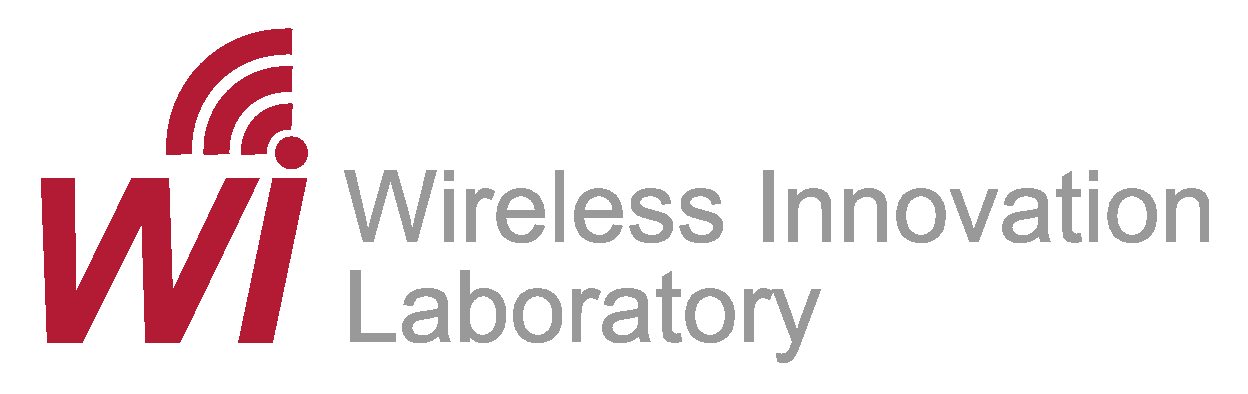
\includegraphics[height=1.125cm]{wilab_logo-A70916.eps} \qquad 
\includegraphics[height=1.125cm]{WPI_Inst_Prim_FulClr.eps}}
% \titlegraphic{\hfill\includegraphics[height=1.5cm]{logo.pdf}}

% Foot for all slides
\setbeamertemplate{frame footer}{\tiny \copyright~2018 by Alexander Wyglinski. This work is licensed under the Creative Commons Attribution-ShareAlike 4.0 International License. To view a copy of this license, visit http://creativecommons.org/licenses/by-sa/4.0/.}

\begin{document}

%\captionsetup[subfigure]{labelformat=empty}

%%%%%%%%%%%%%%%%%%%%%%%%%%%%%%%%%%%%%%%%%%%%%%%%%%%%%%%%%%

\maketitle




%%%%%%%%%%%%%%%%%%%%%%%%%%%%%%%%%%%%%%%%%%%%%%%%%%%%%%%%%%

\frame
{
  \frametitle{What is Carrier Offset?}

   \begin{itemize}
    \item Receiving and transmitting radios run on different local oscillators (LOs)
    \begin{itemize}
     \item LOs responsible for various radio operations, including the implementation of carrier frequency
     \item Differences due to impurities, electrical noise, temperature differences between LOs, etc
     \item LO drift over time
    \end{itemize}
    \item LO differences can result in random phase noise, carrier frequency offset, initial phase mismatch
    \begin{itemize}
     \item We will focus on carrier frequency offset in this lecture
    \end{itemize}
   \end{itemize}



}

%%%%%%%%%%%%%%%%%%%%%%%%%%%%%%%%%%%%%%%%%%%%%%%%%%%%%%%%%%

\frame
{
  \frametitle{Carrier Offset Illustration}

\centering
What happens when we apply a superheterodyne receiver possessing carrier frequency $f_c+\Delta{f}$ to a transmitted signal $s(t)=m(t)\cos(2\pi{f_c}t)$?

}

%%%%%%%%%%%%%%%%%%%%%%%%%%%%%%%%%%%%%%%%%%%%%%%%%%%%%%%%%%

\frame
{
  \frametitle{Describing LO Quality}

  \begin{itemize}
   \item LOs described in parts per million (PPM)
   \begin{itemize}
    \item This translates into maximum carrier offset for given frequency
    \item For example, ADALM Pluto has internal LO rated at 25~PPM
   \end{itemize}
   \item Mathematically, this is defined as:
   \begin{equation}
    f_{o,\max}=\frac{f_c\times{PPM}}{10^6}
   \end{equation}
  \end{itemize}

}

%%%%%%%%%%%%%%%%%%%%%%%%%%%%%%%%%%%%%%%%%%%%%%%%%%%%%%%%%%

\frame
{
  \frametitle{Modeling Carrier Offset}

  \begin{itemize}
   \item Mathematically, this is defined as:
   \begin{equation}
    r(k)=s(k)e^{j(2\pi{f_o}kT+\theta)}+n(k)=s(k)e^{j({\omega_o}kT+\theta)}+n(k)
   \end{equation}
   where $n(k)$ is zero-mean Gaussian random process, $T$ is symbol period, $\theta$ is carrier phase, and $\omega_o$ is carrier frequency offset
  \end{itemize}

}

%%%%%%%%%%%%%%%%%%%%%%%%%%%%%%%%%%%%%%%%%%%%%%%%%%%%%%%%%%
\frame
{
  \frametitle{Relationship between Frequency and Phase}

  \begin{itemize}
   \item Angular frequency $\omega$ is a measure of changing phase $\theta$:
   \begin{equation}
    \omega=\frac{d\theta}{dt}=2\pi{f}
   \end{equation}
   \item Recovering phase of a signal is equivalent to recovering its frequency
   \item Instantaneous phase $\theta$ of any complex signal $x(k)$ can be measured using:
   \begin{equation}
    \theta=\tan^{-1}\left(\frac{\Im(x(k))}{\Re(x(k))}\right)
   \end{equation}

  \end{itemize}

}

%%%%%%%%%%%%%%%%%%%%%%%%%%%%%%%%%%%%%%%%%%%%%%%%%%%%%%%%%%

\frame
{
  \frametitle{Carrier Offset Compensation}

  \begin{itemize}
   \item Various situations might involve carrier frequency offsets that could be potentially very large
   \item For these situations, it is advisable to divide up carrier frequency offset compensation into two parts:
   \begin{itemize}
    \item \textbf{Coarse Frequency Correction}: Tries to find the approximate amount of carrier offset present in a transmission
    \item \textbf{Fine Frequency Correction}: Based on coarse frequency offset compensation, this process obtains precise amount of carrier offset remaining in transceiver
   \end{itemize}
  \end{itemize}

}

%%%%%%%%%%%%%%%%%%%%%%%%%%%%%%%%%%%%%%%%%%%%%%%%%%%%%%%%%%

\frame
{
  \frametitle{Coarse Frequency Correction}

  \begin{itemize}
   \item There exists two types of coarse frequency correction
   \begin{itemize}
    \item \textbf{Data-aided}: Uses correlation type structures that leverage knowledge of received signal, \textit{e.g.}, preamble
    \begin{itemize}
     \item Performance limited by length of preamble
    \end{itemize}
    \item \textbf{Blind} or \textbf{non-data-aided} (NDA): Uses open-loop methodology over duration of transmission to approximately identify carrier frequency offset
   \end{itemize}
  \end{itemize}

}

%%%%%%%%%%%%%%%%%%%%%%%%%%%%%%%%%%%%%%%%%%%%%%%%%%%%%%%%%%

\frame
{
  \frametitle{NDA-Based Coarse Frequency Correction}

  \begin{itemize}
   \item NDA-based coarse frequency correction uses fast Fourier transform (FFT)
   \item Obtains rough estimate on carrier frequency location
   \item Avoid taking peak value resulting from FFT as approximate location of carrier frequency
   \begin{itemize}
    \item This is often not accurate especially if not spectrum not symmetric
   \end{itemize}
  \item Instead, remove modulation components of signal by raising signal to its modulation order $M$, \textit{i.e.}:
  \begin{equation}
   r^M(k)=s^M(k)e^{j(2\pi{f_o}kT+\theta)M}
  \end{equation}
  \begin{itemize}
   \item This will shift offset by $M$ times its original location and make $s(t)$ purely real or imaginary $\rightarrow$ Only a tone will remain
  \end{itemize}
  \item Take FFT bin with highest energy level $\rightarrow$ Tone corresponding to carrier frequency
  \begin{itemize}
   \item Performance of FFT dependent on resolution
  \end{itemize}
  \end{itemize}

}

%%%%%%%%%%%%%%%%%%%%%%%%%%%%%%%%%%%%%%%%%%%%%%%%%%%%%%%%%%

\end{document}
